\chapter{Introduction}
\label{chap:introduction}

The proliferation of cloud storage, content distribution networks, and 
public curated datasets poses new challenges and
opportunities for hosting data.  On the one hand, the availability of
professionally-maintained services is a boon to developers, since it lets them
offload the operational burden of hosting data.  On the other
hand, it is difficult to leverage these services over long
timescales.  Services can appear and disappear, and service operators can
unilaterally change their APIs, pricing, and trustworthiness.
Over long enough timescales, developers find themselves continuously
patching their applications to accommodate new service behaviors.

This thesis presents a novel storage architecture, called \emph{wide-area
software-defined storage} (SDS), that helps developers
leverage these commodity services without this constant patching.
In SDS, developers specify their desired
\emph{end-to-end storage semantics} independently of
both applications and underlying services.  The storage semantics define the
rules for processing application reads and writes, and reside in an architectural
layer ``on top'' of cloud services but ``beneath'' applications.
This thesis presents SDS as an architecture for implementing storage semantics, and
shows how developers can realize the benefits of cloud services without the
long-term risks.

\section{System-of-Systems Approach}

Applications built on cloud services are systems-of-systems.
A \emph{system-of-systems} is a process that aggregates the
functionality provided by multiple independent networked processes
in order to solve a problem that none of them could
handle on their own.  The most prominent system-of-systems 
is the Internet, which uses peering agreements and the Border Gateway
Protocol~\cite{bgp} to aggregate the routing logic in
multiple autonomous networks to provide a global end-to-end packet delivery
service.

Networked processes that run in the Internet's application layer can also
be systems-of-systems.  For example, university Webmail is a
system-of-systems application that 
aggregates DNS, the world's SMTP servers, campus-hosted
Web servers, and a university-wide identity and authentication
system to grant students and faculty access to their email in their Web browsers
(Figure~\ref{fig:chap1-system-of-systems}).  Application-layer systems can be combined with other
application-layer systems to build new application-layer systems.

\begin{figure}[h]
   \centering
   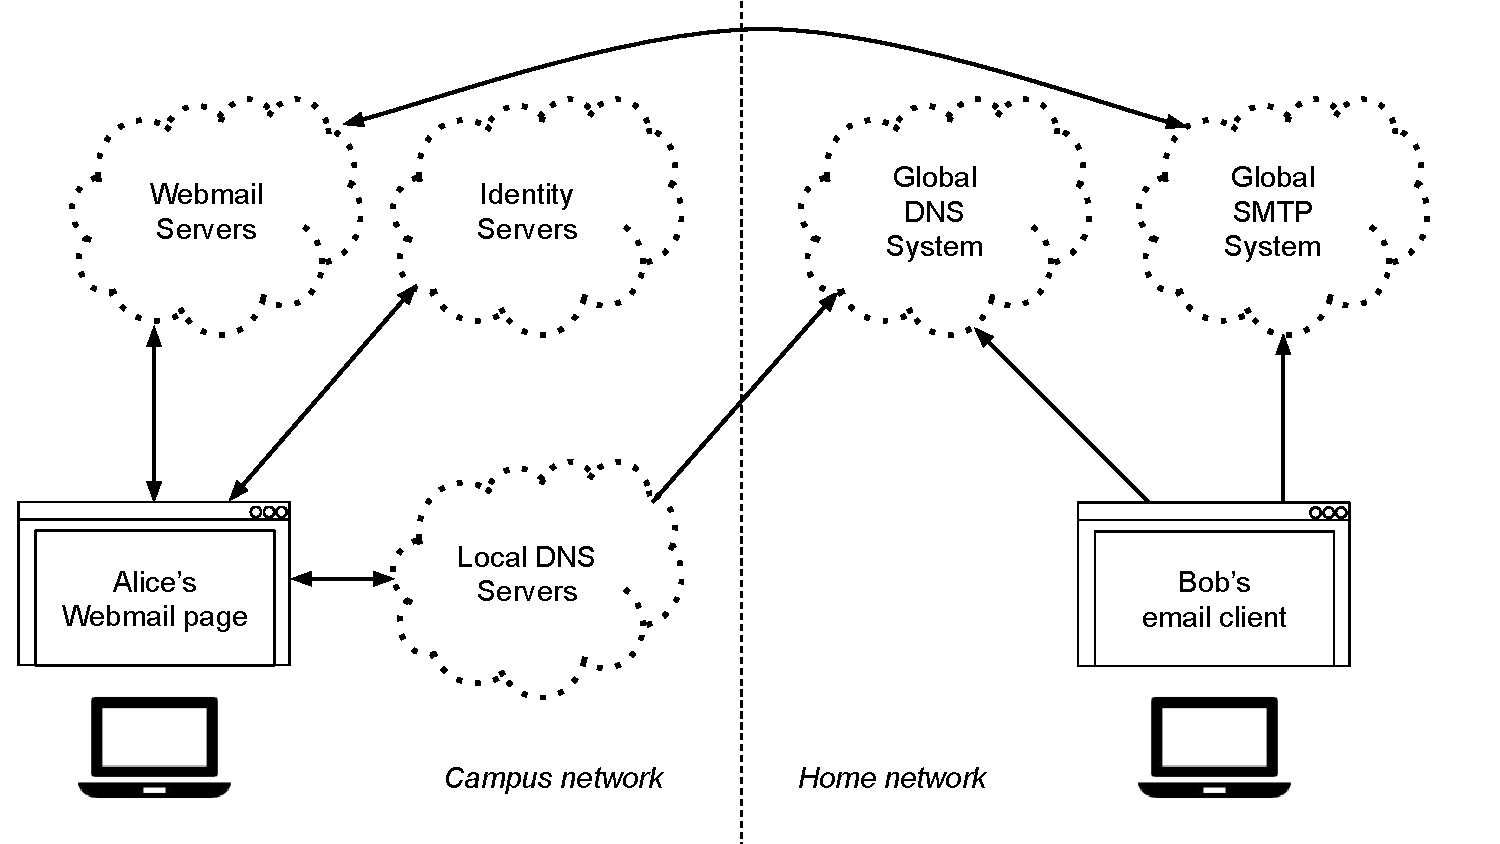
\includegraphics[width=0.9\textwidth,page=1]{figures/dissertation-figures}
   \caption{Webmail is a system-of-systems wide-area application.  In order for
   Alice to receive an email from Bob, her university's DNS and SMTP servers
   must coordinate with the global DNS and SMTP networks, and her university's
   identity service and Webmail servers must coordinate to deliver her mail to
   her Web browser.}
   \label{fig:chap1-system-of-systems}
\end{figure}

This thesis is concerned with helping developers build
system-of-systems applications on top of third-party \emph{cloud storage},
\emph{content distribution networks} (CDNs), and \emph{curated data-sets}.
Cloud storage acts as the read/write storage medium for the
application's state.  CDNs help applications overcome high latencies and
bandwidth bottlenecks in WAN settings by serving downstream readers cached data.
Curated datasets host read-only data on behalf of a set of applications, providing value
to each one without requiring them to individually go out and
collect data.

These three types of services are of interest because they implement a
minimal set of requirements for many more applications and services.  For
example, the application and service offerings from Google are
realized with shared corporate cloud storage (i.e. Megastore~\cite{megastore},
Spanner~\cite{spanner}, GFS~\cite{gfs}), a shared corporate
CDN~\cite{google-cdn}, and multiple shared repositories of user behavioral data
that assist in machine-learning tasks like 
spam fighting, page ranking, voice recognition, and so on.  Google's public application
platforms are built with these services as
well~\cite{google-appengine}~\cite{google-cloud}.  The situation is similar for
Amazon AWS and Facebook, which use a common core of cloud storage, CDNs, and
curated datasets to implement both their applications and 
higher-level services (like ad placement and logging).

Most applications are not built on top of bespoke datacenters, CDNs, and curated
datasets, but instead rely on third-party service offerings.  The developer
leases service capacity in order to build their applications.
For example, a navigation application
would host its users' preferred routes, maps, and historic queries in cloud storage,
use a CDN to cache map data in appropriate geographic regions,
and use public weather data aggregated by NOAA~\cite{noaa} and crowdsourced road
data from OpenStreetMap~\cite{openstreetmap} to determine the best route to take.
As another example, a movie streaming service like Netflix~\cite{netflix} would
host its users' streaming history in cloud storage, use a CDN to accelerate the
delivery of popular media, and curate the catalog of movies as a shared dataset
for its mobile and Web applications.

% why these three?  can we think of production examples?
% * facebook: datacenters for storage, fbcdn for delivery, social graph for 3rd
% party integration
% * google; datacenters for storage, google CDN for delivery, website index and
% user ad behavior for AI applications

% another example: AI/ML datasets

% TODO: numbers from e.g. Gartner about the growth of the cloud services market?
The growth of these public commodity cloud services and the proliferation of
applications using them demonstrates their promise as system-of-systems
building blocks.  Developers do not have to re-invent existing functionality
each time they build a new application.  Instead, they can
purchase metered service capacity to handle their applications' needs.
This reduces time-to-market, speeds up product iteration, externalizes
infrastructure maintenance and costs,
and lowers the barrier to entry for building new applications.

The difficulty with this approach is that \emph{developers spend lots of
time and effort preserving end-to-end storage semantics}.  This is because an application's
storage semantics depend on the semantics of each cloud service it uses.

To build a correct implementation, developers must account for
the semantics of their chosen services in the application's design.
For example, the aforementioned navigation application's servers
must coordinate with downstream CDN servers to ensure that
clients read fresh data.  As another example, the Web servers in the
campus Webmail application must coordinate with 
the authentication servers to enforce campus-wide access controls.
These concerns are not part of the business logic of the applications, but 
nevertheless must be addressed in order for the application to behave correctly.

\subsection{Challenges}

% government institutions can't use 3rd party clouds (cite conversation)
% is there a law we can cite? a policy doc?
% * FERPA for student data
This thesis addresses the challenges of preserving end-to-end storage semantics
in wide-area applications built from third-party cloud services.  Three specific
pain-points are identified.

First, \emph{developers have no control over the services' semantics}.
Cloud services can unilaterally
change their pricing, feature-set, APIs, semantics, availability, and
trustworthiness.  Applications that rely on a service can break unexpectedly
when the service changes its behaviors, and in doing so,
cost developers unforeseeable amounts of time and money.

Developers agree to this one-way relationship when accepting the service's terms of service.  The terms of
service for popular services explicitly state that the operators have the ability to affect unilateral
changes.  For example, Dropbox unilaterally broke its API from version 1 to version
2~\cite{dropbox-v2-api-psa}, and both Twitter and Instagram dropped API
endpoints even after non-trivial
applications were built to leverage
it~\cite{twitter-api-deprecation-psa}~\cite{instagram-api-drop}. % TODO: find a better reference for this

The second challenge is that \emph{cloud services are heterogeneous}, which
makes it hard to change both services and end-to-end semantics once the application is deployed.
In practice, services that fill similar roles do not always offer the same semantics.
For example, a service designed to use Amazon S3 may 
depend on its sequential consistency, which may prevent the developer from
switching to Microsoft OneDrive (which provides eventual
consistency~\cite{consistency-comparison-cloud-storage}) even though both
services fulfill a cloud storage role.   % https://blog.cloudrail.com/compare-consistency-models-of-cloud-storage-services/

Without careful planning, the application can become tightly coupled
to its services by accidentally relying on undocumented or unacknowledged
behavior.  This creates high service switching costs, making it
difficult for developers to move the application to better
offerings or change the application's semantics later to meet new requirements.

The third challenge is that application users have
certain expectations about how their data will be used, and which data
they will interact with.  The application must
meet these expectations in order to be usable.  However, a users' expectations are
specific to each application, each datum, and to other users.  They can be
arbitrarily specific, but some common example include:

\begin{itemize}
   \item Data privacy.  Users may expect that their data will be visible only to
      people they designate.
   \item Data non-repudiability.  Users may expect that their
      data or the data they read from other users is non-repudiable and will not
      be erased by the application.
   \item Data blocking.  Users may expect the application to silently prevent
      other users' data from reaching them.  This is especially relevant to
      forums and social media applications, which must contend with online
      harassment.
   \item Data portability.  Users may expect that they will be able to download
      their data from the application at some point in the future and use it in
      another application.
   \item Access audits.  Users may expect that the application will tell them
      how their data has been used, as well as when and where it was used.
   \item Ancillary data.  Applications generate data from user behavior, and
      users may expect to be able to read it.  For example, Facebook will tell
      users which third-party advertisers may send them ads.
   \item Data retention.  Users may expect that the application holds on to data
      they delete for a certain amount of time, so they can un-delete it.  For
      example, Gmail~\cite{gmail} implements a ``trash can'' abstraction that retains
      deleted emails for 30 days after they are deleted from the user's inbox.
   \item Data amnesia.  Users may expect that the data they delete will be
      erased and forgotten by the application.
   \item Legal compliance.  Users may expect that access to their data will be
      governed under a particular jurisdiction, i.e. the one that they live in,
      the one in which their data replicas reside, and so on.
\end{itemize}

This is not an exhaustive list by any means, but is meant to illustrate the point
that developers need to honor their users' expectations, or risk alienating
their users and/or suffering legal consequences.  This thesis
refers to a machine-readable encoding of the user's expectations for their data
in a particular application as the user's \emph{data-hosting policy}.

Today, applications encode and globally enforce data-hosting policies by means of
a ``settings page'' for users, which gives users some levers to control how
their data will be used.  For example, most social media applications have an
``Account Privacy'' page that lets the user control which other users can access
which data.  As another example, government regulations like
GDPR~\cite{gdpr} require applications to provide an ``export data'' page for
downloading all of the user's data, as well as a ``delete and forget'' page for
permanently erasing the data.

In the system-of-systems approach, the application alone cannot be trusted to
enforce all data-hosting policies.  This is because the data records are stored in
third-party service providers that are unaware of the policies, and may
do things that violate them.  The developers have no recourse if this happens.

The third challenge that developers of system-of-systems applications have to overcome is
that \emph{data-hosting policies must be enforced by the user's
organizations while preserving the end-to-end storage semantics}.
For the purposes of this thesis, an \emph{organization} is an
autonomous set of computers that a user uses to interact with their data 
in a particular application.  Example organizations include a
user's personal devices, a corporation's workstations, or a lab's
computer cluster. 

If a user cannot rely on the application or storage provider
to enforce her policy, then she must rely on her organization to do so on her behalf.
This means that each organization needs to be free to
set and enforce data-hosting policies on their users' behalf,
and developers need to ensure that each policy's
rules are followed without affecting the end-to-end storage semantics.
This is true of the example Webmail application, since the campus-hosted
servers, the SMTP servers, and the DNS servers can each
decide how they store and serve their message and routing information
without affecting the store-and-forward semantics of email.

The difficulty of building cross-organization system-of-systems applications arises from the
degree to which organizations are willing to trust other organizations to enforce
their users' policies.  This degree of trust falls on a spectrum.
At one extreme, users of an organization do not trust other organizations with
their policy enforcement at all.  The designs of applications at this extreme reflect this by requiring
each organization to host their users' data (including choosing their own compliant storage
providers, if any), thus putting them in a position to
mediate all accesses to it.
The campus Webmail example falls into this extreme, as do most federated
applications like IRC~\cite{irc}, XMPP~\cite{xmpp},
Diaspora~\cite{diaspora}, and Mastodon~\cite{mastadon}.

At the other extreme,
users fully trust external organizations.
The designs of applications at this extreme allow each organization to completely delegate
policy enforcement to another organization.  Examples include most Web services like 
Facebook~\cite{facebook}, Google Apps~\cite{gapps}, and Microsoft
Office 365~\cite{microsoft-apps}, where each user completely trusts the company running
the application to enforce her data policies.

At both extremes, policy enforcement mechanisms are
straightforward to develop.  When the organization hosts the user's data, the user 
instructs their organization on when reads and writes from other
organizations are permitted and when they are denied.
For example, the campus Webmail application lets university users
control read access to their inboxes by requiring passwords, and lets
them control write accesses both by requiring passwords to send mail
and by allowing users to
set spam filter rules that constrain which inbound messages
(i.e. ``writes'' from other users) they will
see.  At the other extreme when the user completely trusts an external organization to enforce her
data-hosting policies, the developer simply provides an ``account settings''
feature that lets the user control which reads and writes to her data are
permitted by other users, and how to authorize them.

However, system-of-systems applications built on cloud services
fall in-between these two extremes.  In these applications, the data policy
enforcement mechanisms are \emph{partially} deployed in the same
organization that hosts the data, but not completely.  In these cases,
organizations at a minimum trust the cloud services to keep their data available.
They may also trust them with additional
responsibilities on a case-by-case basis,
such as domain-specific access controls or replica placement.

The challenge to developers is to accommodate the \emph{whole spectrum} of
users' trust relationships with organizations and cloud services.
Each organization not only has different user-given data-hosting
policies, but also has different degrees of trust in the cloud service and other
organizations with respect to enforcing them.
This affects the design of these applications such that in the limit,
the application must be aware of each trust relationship and each policy that
exists.  This poses a problem to developers, since developers 
must provide the appropriate mechanisms for enforcing them while still
preserving end-to-end storage semantics.

% DONE
% add a subsection: problem statement (crisp statement)
% make sure chapter 2's objectives tightly link to this problem statement
% distilled design principles: link back to this problem statement
% goal: be able to read 1.1.1, 1.1.2, 2.1, and 2.9, and "get it".
% challenges and objectives are *duals* of each other.
% requirements are derived from objectives, but one layer deeper.
% 2.3-2.8 are the meat.
% 2.9 connects the dots, back to the challenges.
\subsection{Problem Statement}

Building applications on cloud services forces developers to solve two hard
problems in practice.

\begin{itemize}
   \item \textbf{Preserve end-to-end storage semantics}.  This is difficult
      today because developers do not
      control the services' storage semantics.  The services can change their
      behavior, the developers can change the services the application uses, and
      the developers can change the semantics of the application.
      The consequences are the same in all cases:  the developers need to patch the application to
      accommodate the new semantics.

   \item \textbf{Preserve organizational autonomy}.  This is difficult today
      because applications run across multiple organizations and cannot enforce
      data-hosting policies on their own.  However, each organization has its
      own user-given policies that govern what can be done with its users' data.
      Ensuring that each organization is free to enforce its users' policies is
      hard because neither the developers nor the organizations
      control the services' behaviors, and users have varying degrees of trust in
      each service's ability to accommodate their policies.  Moreover, any mechanisms
      that organizations employ to enforce their users' policies must be
      compatible with the application's end-to-end storage semantics.
\end{itemize}

As a result, developers spend a lot of time and effort patching their
application just to keep it running, and cannot realistically honor
each user's data-hosting policies.  This in turn hurts users, since it
limits the extent to which they can safely use the application.  Users are put
into the awkward position of having to avoid using the application, or put
themselves at risk by trusting the application with their data more than they
would like.  This thesis shows developers how to
address both problems in a way that requires minimal additional work once the
application is deployed.

\section{Wide-area Software-defined Storage}

% TODO: this is too brief...show examples above?
% TODO: won't applications run the same risks with SDS as they do with cloud
% services?  can we argue that SDS is somehow more stable than these services?

To address these problems, this thesis presents a 
storage architecture that separates storage semantics
from both cloud services and applications.  The rules for processing reads and writes
are placed in a common data-exchange
layer in-between applications and the cloud services.  A system that
implements this layer is called a \emph{wide-area software-defined storage} (SDS) system
(Figure~\ref{fig:chap1-sds-overview}).

\begin{figure}[h]
   \centering
   \includegraphics[width=0.9\textwidth,page=28]{figures/dissertation-figures}
   \caption{Software-defined storage acts as an intermediate ``narrow waist''
   layer that preserves application-specific storage semantics on top of
   commodity cloud services.}
   \label{fig:chap1-sds-overview}
\end{figure}

SDS systems preserve end-to-end storage semantics on top of cloud services while respecting
organizational autonomy.  A SDS system accommodates changes in service semantics
by encapsulating service-specific interfacing logic inside a ``service driver.''
The service driver gives the SDS system a very simple API for loading and
storing immutable chunks of data.  This isolates a particular service from the rest of the
system and makes its functionality accessible via a common API.  Once the SDS system has a
driver implementation for a service, any SDS-powered application can use it
automatically.

SDS preserves organizations' autonomy without compromising end-to-end semantics by
allowing each user to control the network paths their data takes from the
application's users to the services (and vice versa).  Each organization runs its own
service driver instances for storing its data, and developers supply an
``aggregation driver'' that applies the application-specific storage semantics
over the services used when processing a read or write.

The aggregation driver is an SDS-specific programming concept that developers
use to implement end-to-end storage semantics.  Its
programming model borrows from both the UNIX shell programming and software-defined
network programming paradigms.  The developer writes an aggregation driver as a
series of composable ``stages,'' which are evaluated in sequential order by the
SDS system to process a read or write according to the desired semantics.
Each organization runs one or more aggregation driver stage instances.

Users apply their data-hosting policies by choosing which organizations' service
drivers and aggregation driver stages will carry out the read or write.  The
user does this by selecting the routes that a read or write on a piece of data
is allowed to take through the set of organizations.  In doing so, users choose
which organizations process their reads and writes without violating
application-specific storage semantics.

SDS systems avoid the problem of service lock-in by means of a ``gateway''.
Each organization runs their service drivers and aggregation driver stages
within SDS gateways they control, and the SDS system uses the user's policy
to route reads and writes to her data through a valid sequence of gateways 
in order to preserve end-to-end storage semantics.
Each gateway implements the storage API of the
organization's choice, and serves as the application's access point to the SDS
system.  This allows each organization to choose which APIs are exposed to their
users' applications, and enables each organization to make its own decisions on how
other users read and write its users' data.

\begin{figure}[h]
   \centering
   \includegraphics[width=0.9\textwidth,page=33]{figures/dissertation-figures}
   \caption{Overview of the relationship between service drivers, aggregation
   drivers, and gateways on a read request.  The application's request ``read \texttt{foo}'' is
   processed by a sequence of three aggregation driver stages before
   \texttt{foo}'s data is returned.  The SDS system ensures that each stage is
   executed in the right sequence (preserving semantics),
   and each organization runs a service driver to loads and stores the
   necessary data to do so (preserving autonomy).}
   \label{fig:chap1-sds-implementation-overview}
\end{figure}

The resulting system solves both problems
(Figure~\ref{fig:chap1-sds-implementation-overview}).
It ensures that all reads and writes pass through the
correct sequence of aggregation driver
stages, thereby preserving the end-to-end semantics.  Each stage
loads and stores raw data from the underlying services as needed
by invoking its gateway's service driver(s).  Service drivers may take advantage
of any service-specific features to load and store data, but are required to
expose data to aggregation driver stages as a set of immutable,
content-addressed write-once read-many chunks.  In doing so, SDS separates
application semantics from the semantics of the underlying services while still
allowing developers to take advantage of any useful service-specific
features they offer.

At the same time, users 
control which organizations' aggregation driver stages and service driver
instances are utilized to process a given request.  Moreover, they can control
which gateway instances are selected to process reads and writes.  This yields a way to
translate a user's data-hosting expectations into a
machine-readable data-hosting policy:  they are realized as a set of source
routes on each of the user's data.  By translating policy enforcement into
a source-routing problem, organizations can automatically
preserve its users data-hosting expectations without
violating end-to-end storage semantics.  The user selects gateways that process
their reads and writes in a way that meets their policy's terms.
A detailed description of how service drivers, aggregation
drivers, and gateways coordinate to achieve this is presented in
Chapter~\ref{chap:design_principles}.

\section{Contributions}

The architecture put forth in this thesis is informed by two real-world SDS
implementations and three sample applications.  The implementations were 
designed to accommodate two sets of real-world use-cases: scientific computing,
and ``serverless'' Web applications (i.e. Web applications that can operate
without application-specific servers).
The design principles in this thesis 
were formulated once the implementations were tested and
deployed in production settings.  This thesis claims the following contributions:

\begin{itemize}

\item This thesis presents the design principles of wide-area software-defined storage, framed in
terms of prior work and the real-world storage needs of existing applications.
Adhering to these design principles reduces the man-hours required to keep applications compatible
with existing services while both preserving end-to-end storage semantics and
respecting each organization's data-hosting policies (Chapter~\ref{chap:design_principles}).

\item This thesis presents the design and implementation of two SDS systems: Gaia and
Syndicate.  Syndicate is a real SDS system being deployed in scientific
workflows today, and Gaia is a real SDS system being deployed to build
serverless Web applications.
This thesis uses Gaia and Syndicate to show how to translate SDS design
principles into real systems.
(Chapter~\ref{chap:syndicate_sds}).

\item This thesis shows how to build SDS-powered applications.  The design and
implementation of non-trivial SDS-powered applications \emph{that could not
have been feasibly built without SDS} are presented.  Among these are an end-to-end encrypted
Webmail client that removes the user from key management, a server-less
groupware application that lets users control how their data gets hosted and
accessed, and a scientific data-staging application that
automatically makes fresh datasets available from existing data repositories to
HPC clusters via commodity CDNs.
(Chapter~\ref{chap:applications}).

\item This thesis presents microbenchmarks for Gaia and Syndicate.  The
microbenchmarks show the various overheads of these SDS implementations
impose by processing reads and writes by passing them through aggregation
and service drivers.  The results show that the SDS
systems are efficient at processing larger I/O requests, and that developers
have many options available to influence end-to-end read and write performance.
(Chapter~\ref{chap:evaluation}).

\end{itemize}

These contributions support the thesis that developers can both preserve
end-to-end storage semantics and respect organizational autonomy when building
on cloud services.  A properly-designed SDS system achieves this by framing the
problem in terms of service drivers and aggregation drivers, which can be
written once and reused across applications.  In doing so, SDS systems minimize the amount of
work required to keep an application running.

% TODO: reinforce/tie back to end-to-end storage semantics
% "these four contributions support the thesis that a properly-designed SDS
% system preserves end-to-end semantics..."


